\chapter{Resultados}\label{CAP7}

\section{Visualizador}
        En esta sección se presentan los resultados de la visualización del robot delta en Rviz. Primero se muestra la explicación gráfica de la conexión de los nodos y temas creados en ROS. Luego se muestran los enlaces y los marcos referencia de cada enlace en coordenadas TF. 

    \subsection{Temas y Nodo}
    
    \begin{figure}[h]
            \centering
            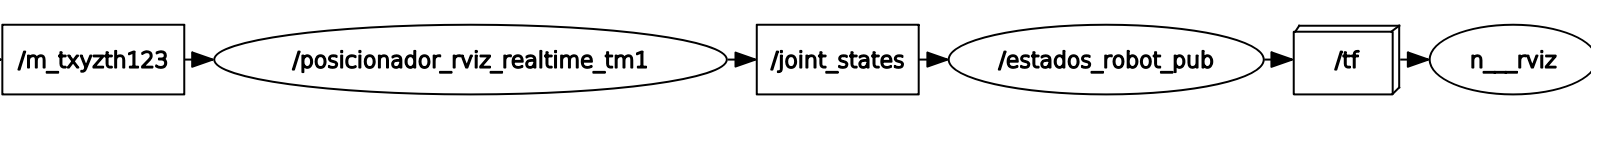
\includegraphics[width=1.0\linewidth]{Main/Chapter7/Images7/nodo_1.png}
            \caption{Rrrrrrrrrrrrrrrrrrrrrrrrrrrrrrrrrrrrrrrrrrrrrrrrrrrrrrrrrrrrrrrrrrr}
            \label{f:cap7_rviz1111}
        \end{figure} 
        
    \begin{itemize}
        \item {\textbf{Entrada:} el tema 'm\_txyzth123' esta configurado por un mensaje escrito en el archivo llamado 'matriz\_path\_ls.msg', compuesto por los datos de la tabla \ref{tab:cap6_rviz_1_msg}. Las matrices x,y,z son los puntos de la trayectoria lineal  en el espacio cartesiano de la base movil. Las matrices th1,th2,th3 son la trayectoria en el espacio articular de los actuadores. La matriz de tiempo es la escala de tiempo de la trayectoria a simular.}
        \item {\textbf{Nodo:} el nodo con el nombre 'posicionador\_rviz\_realtime\_tm1' es el encargado de calcular los ángulos de las articulación o juntas del robot delta a partir de las coordenadas en el espacio cartesiano xyz  de la trayectoria de la base móvil. Los puntos xyz son utilizados para simular el movimiento la base movil y los angulos de cada junta para el movimiento de 3 cadenas cinemáticas.}
        \item {\textbf{Salida:}  el tema 'joint\_states' esta configurado por un mensaje escrito en el archivo llamado 'JointState.msg', compuesto por los datos mostrados en la tabla \ref{tab:cap6_rviz_2_msg}. Este es un mensaje que contiene datos para describir el estado de un conjunto de juntas controladas por torque. Cada articulación (revoluta o prismática) se identifica de forma única por su nombre. Name es el nombre de cada articulación, position es la posición de la articulación (rad o m), velocity es la velocidad de la articulación (rad/s o m/s) y effort es el esfuerzo que se aplica en la articulación (Nm o N). En esta tesis solo se utilizan las matrices de los nombres y posición de cada junta.}
    \end{itemize} 
    
        \begingroup
            \renewcommand{\arraystretch}{1.5}
            \begin{table}[H]
                \centering
                \begin{tabular}{c m{2.5cm}}
                   \hline                   \hline
                   \textbf{Tipo de dato}  & \textbf{Nombre}    \\\hline \hline 
                   bool &  permiso
                   \\\hline
                   int64 &  id\_call
                   \\\hline
                   float32[] &  x
                   \\\hline
                   float32[] &  y
                   \\\hline
                   float32[] &  z
                   \\\hline
                   float32[] &  th1
                   \\\hline
                   float32[] &  th2
                   \\\hline
                   float32[] &  th3
                   \\\hline
                   float32[] &  tiempo
                      \\\hline                   \hline
                \end{tabular}
                \caption{Referencias del dibujo}
                \label{tab:cap6_rviz_1_msg}
            \end{table}
        \endgroup
        
        \begingroup
            \renewcommand{\arraystretch}{1.5}
            \begin{table}[H]
                \centering
                \begin{tabular}{c m{2.5cm}}
                   \hline                   \hline
                   \textbf{Tipo de dato}  & \textbf{Nombre}    \\\hline \hline 
                    string[]  & name
                   \\\hline
                    float64[]  & position
                   \\\hline
                    float64[]  & velocity
                   \\\hline
                    float64[] &  effort
                    \\\hline                   \hline
                \end{tabular}
                \caption{Referencias del dibujo}
                \label{tab:cap6_rviz_2_msg}
            \end{table}
        \endgroup

\newpage

    \subsection{Enlaces y Juntas}\label{enalcesyjuntas_cap7}
        La figura \ref{f:cap7_rviz_2} representa la visualización de los enlaces del robot delta. La base fija es un cilindro de color gris, la base móvil es un cilindro de color azul y tanto los brazos como los antebrazos son cajas alargadas de color blanco. Además, se muestra los nombres de cada enlace con sus marcos de referencia TF respectivos.
        \begin{figure}[h]
            \centering
            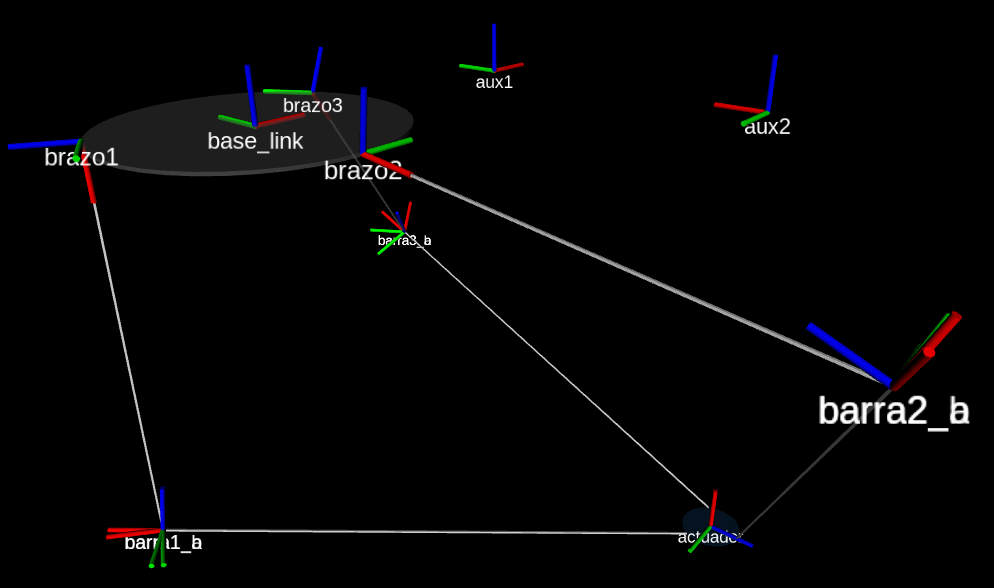
\includegraphics[width=0.8\linewidth]{Main/Chapter7/Images7/rviz_2.png}
            \caption{R}
            \label{f:cap7_rviz_2}
        \end{figure}  
        
    La figura \ref{f:cap7_rviz_3} se muestra la relación entre cada enlace, es decir, la relación padre-hijo. Se aprecian 4 cadenas cinemáticas las cuales son: 3 compuestas por la base fija-brazo-antebrazo y 1 compuesta por la base móvil.    
    \begin{figure}[h]
            \centering
            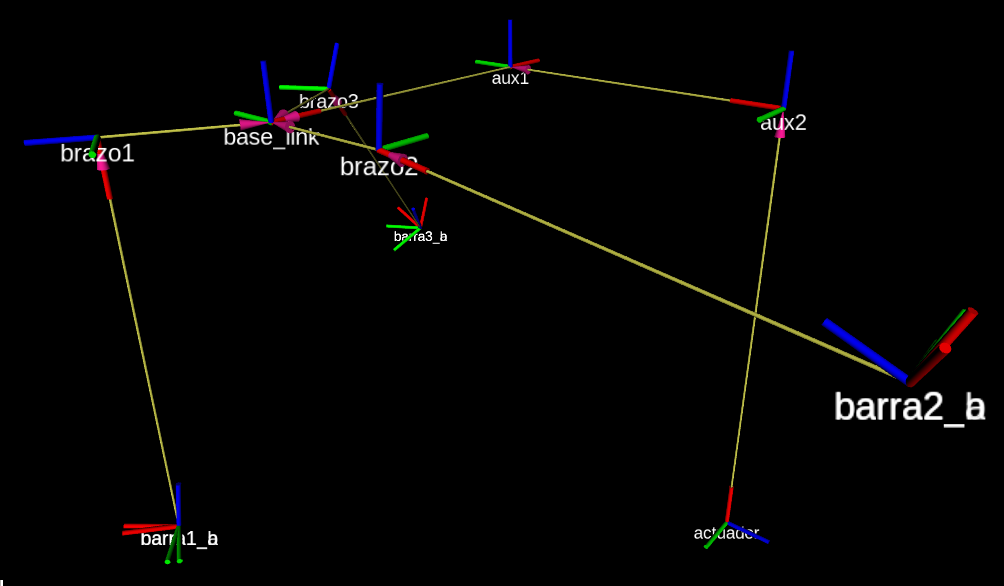
\includegraphics[width=0.8\linewidth]{Main/Chapter7/Images7/rviz_3.png}
            \caption{Rrrrrrrrrrrrrrrrrrrrrrrrrrrrrrrrrrrrrrrrrrrrrrrrrrrrrrrrrrrrrrrrrrr}
            \label{f:cap7_rviz_3}
        \end{figure}  

\newpage

    \subsection{Estructura de arbol URDF}
    La estructura de árbol URDF es una representación gráfica de la relación padre-hijo entre los enlaces y sus marcos de referencia. En la figura \ref{f:cap7_rviz_12341} los nombre de los enlaces son los en rectángulos blancos y las juntas en círculos azules. Las juntas son las encargadas de configurar la relación padre-hijo. En la figura ,xyz se refiere a la traslación del marco de referencia de los hijos respecto al marco de referencia del padre, de modo similar, rpy es la rotación del marco de referencia de los hijos respecto a los de los padres. Al igual que en la sección \ref{enalcesyjuntas_cap7}, se aprecian 4 cadenas cinemáticas.

        \begin{figure}[h]
            \centering
            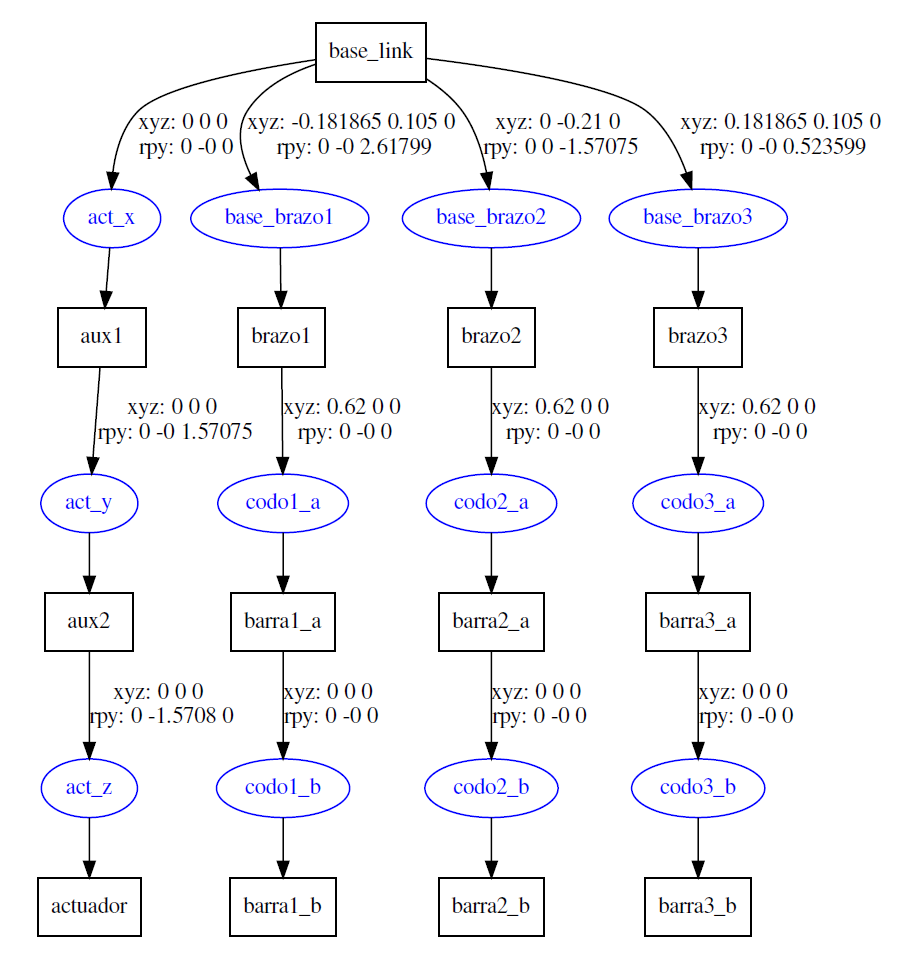
\includegraphics[width=1.0\linewidth]{Main/Chapter7/Images7/rviz_1.png}
            \caption{RRrrrrrrrrrrrrrrrrrrrrrrrrrrrrrrrrrrrrrrrrrrrrrrrrrrrrrrrrrrrrrrrrrr}
            \label{f:cap7_rviz_12341}
        \end{figure}  
    
\newpage


\section{Espacio de Trabajo}
        En esta sección se presentan los resultados del espacio de trabajo del robot delta del capitulo \ref{CAP6} con las restricciones impuestas en la tabla \ref{t:cap6_ws_1}
        
    \subsection{Temas y Nodo}
    
        \begin{figure}[h]
            \centering
            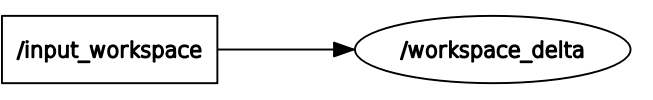
\includegraphics[width=1.0\linewidth]{Main/Chapter7/Images7/nodo_2.png}
            \caption{Rrrrrrrrrrrrrrrrrrrrrrrrrrrrrrrrrrrr}
            \label{f:cap7_rviz2222}
        \end{figure}    
    
    \begin{itemize}
        \item {\textbf{Entrada:}  el tema 'input\_workspace' esta configurado por un mensaje escrito en el archivo llamado 'parameter\_ws.msg', compuesto por los datos de la tabla \ref{tab:cap6_rviz_4_msg}. Step es la discretizacion de los ángulos de los motores en grados para graficar el espacio de trabajo. Graficar\_realtime es una entrada que confirma si se quieren graficar los resultados del espacio de trabajo. }
        \item {\textbf{Nodo:} workspace\_delta es el nodo encargado de generar el espacio de trabajo del robot delta a partir de restricciones impuestas.}
    \end{itemize}
    
        
            \begingroup
            \renewcommand{\arraystretch}{2.0}
            \begin{table}[H]
                \centering
                \begin{tabular}{c m{3.0cm}}
                   \hline                   \hline
                   \textbf{Tipo de dato}  & \textbf{Nombre}    \\\hline \hline 
                    bool & graficar\_realtime
                   \\\hline
                    int64 & step
                    \\\hline                   \hline
                \end{tabular}
                \caption{Referencias del dibujo}
                \label{tab:cap6_rviz_4_msg}
            \end{table}
        \endgroup    
        
        \newpage

        \subsection{Espacio de trabajo}
        \begin{figure}[h]
            \centering
            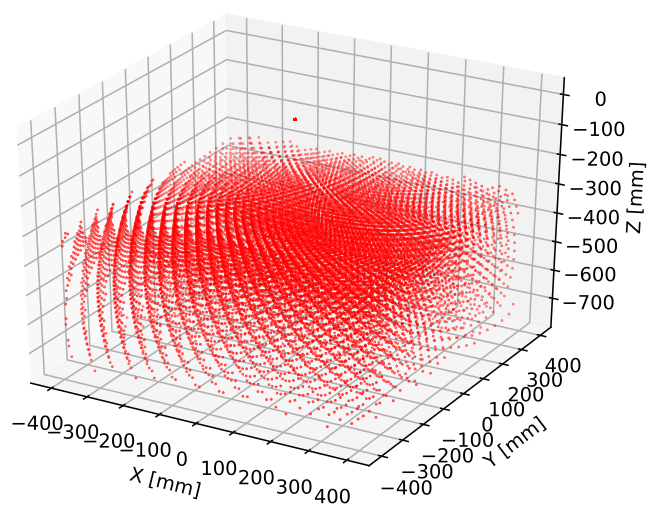
\includegraphics[width=0.55\linewidth]{Main/Chapter7/Images7/ws_6.png}
            %\includesvg[width=1\textwidth]{Main/Chapter7/Images7/ws_6.svg}
            \caption{R}
            \label{f:cap7_ws6}
        \end{figure}
        
    \subsection{Puntos Alcanzables}
        \begin{figure}[h]
            \centering
            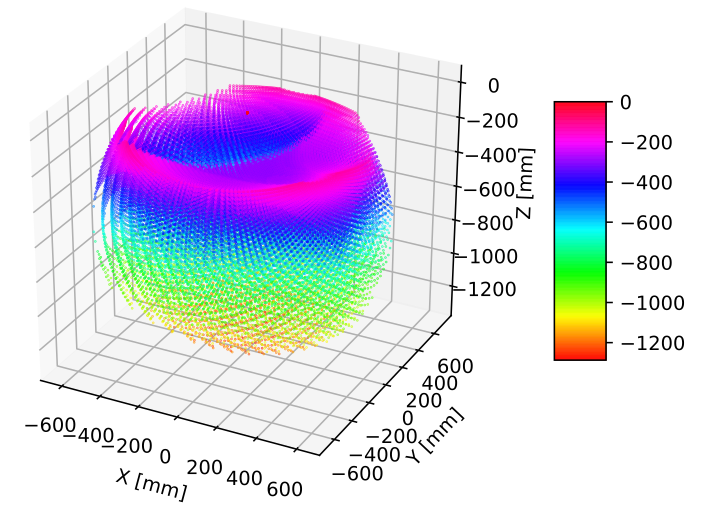
\includegraphics[width=0.82\linewidth]{Main/Chapter7/Images7/ws_1.png}
            %\includesvg[width=1\textwidth]{Main/Chapter7/Images7/ws_1.svg}
            \caption{R}
            \label{f:cap7_ws1}
        \end{figure}    
        
    \newpage

    
    \subsection{Proyección plano $XY$}
        \begin{figure}[h]
            \centering
            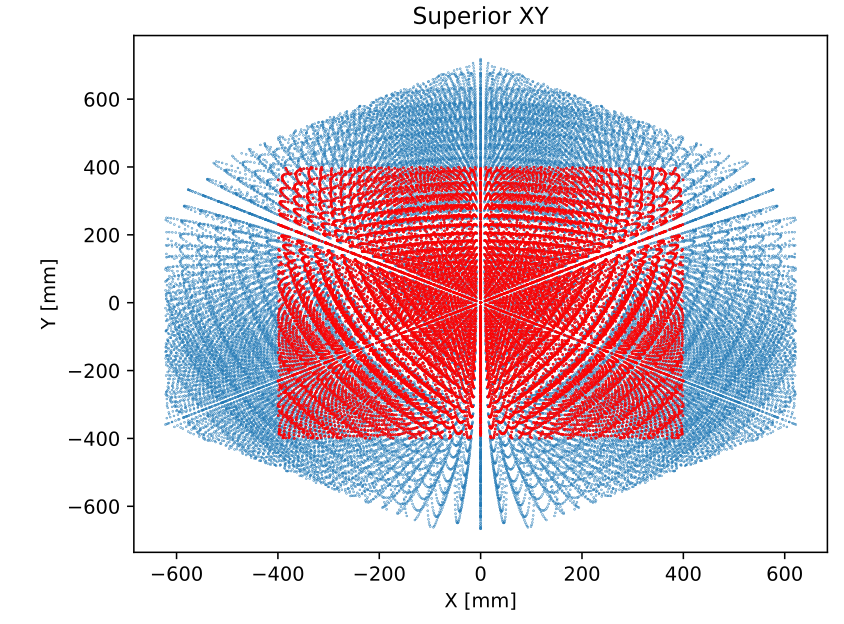
\includegraphics[width=0.65\linewidth]{Main/Chapter7/Images7/ws_2.png}
            %\includesvg[width=1\textwidth]{Main/Chapter7/Images7/ws_2.svg}
            \caption{R}
            \label{f:cap7_ws2}
        \end{figure}  
    
    \subsection{Proyección plano $XZ$}
        \begin{figure}[h]
            \centering
            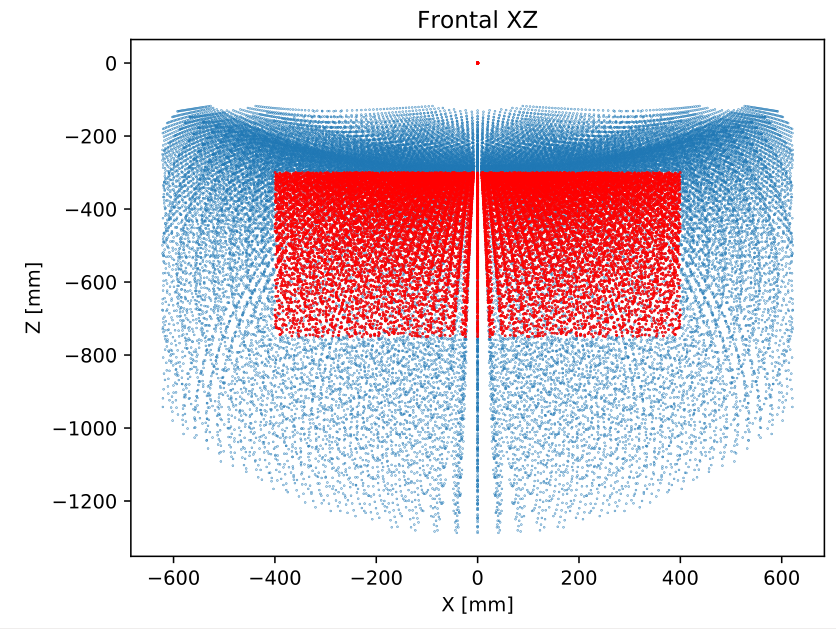
\includegraphics[width=0.65\linewidth]{Main/Chapter7/Images7/ws_3.png}
            %\includesvg[width=1\textwidth]{Main/Chapter7/Images7/ws_3.svg}
            \caption{R}
            \label{f:cap7_ws3}
        \end{figure}  
        
    \newpage
    
    \subsection{Singularidad $J_{x}$}
        \begin{figure}[h]
            \centering
            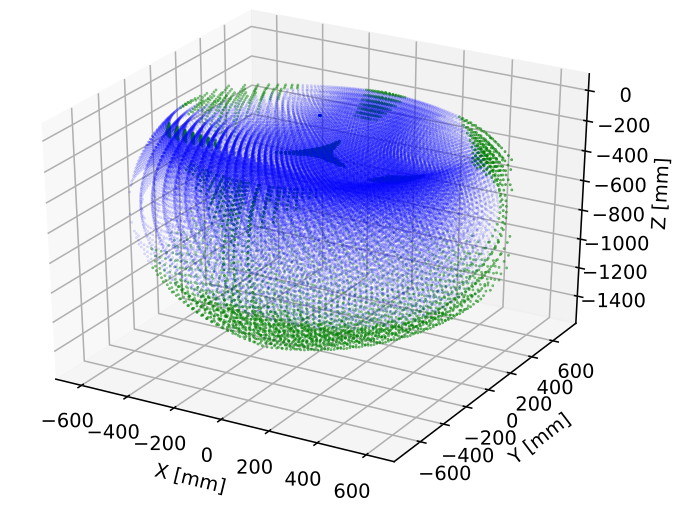
\includegraphics[width=0.65\linewidth]{Main/Chapter7/Images7/ws_4.png}
            %\includesvg[width=1\textwidth]{Main/Chapter7/Images7/ws_4.svg}
            \caption{R}
            \label{f:cap7_ws4}
        \end{figure}  
    
    \subsection{Singularidad $J_{\theta}$}
        \begin{figure}[h]
            \centering
            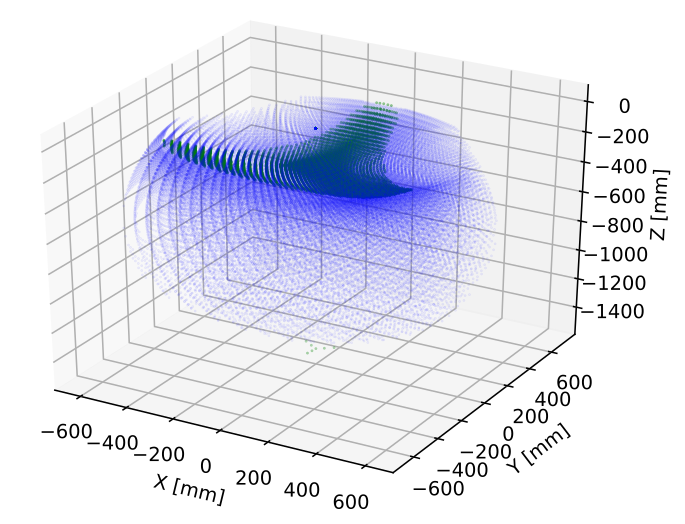
\includegraphics[width=0.65\linewidth]{Main/Chapter7/Images7/ws_5.png}
            %\includesvg[width=1\textwidth]{Main/Chapter7/Images7/ws_5.svg}
            \caption{R}
            \label{f:cap7_ws5}
        \end{figure}  
        
    \newpage
    


        
        
        
        
\newpage


\section{Trayectorias}
    En esta sección se presentan los resultados de los torques aplicados a los actuadores del robot delta del capitulo \ref{CAP5} para realizar las trayectorias impuestas de la sección \ref{nodoprincipal_tray}.

    \subsection{Temas y Nodo}
    
    \begin{figure}[h]
            \centering
            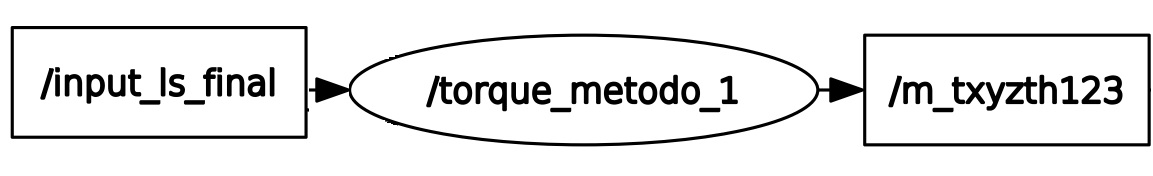
\includegraphics[width=1.0\textwidth]{Main/Chapter7/Images7/nodo_3.jpg}
            \caption{Resultado de la dinámica inversa en trayectoria 1}
            \label{f:cap7_tray_5_nodo}
    \end{figure}
    
    \begin{itemize}
        \item {\textbf{Entrada:}  el tema 'input\_workspace' esta configurado por un mensaje escrito en el archivo llamado 'parameter\_ws.msg', compuesto por los datos de la tabla \ref{tab:cap6_rviz_4_msg}. Step es la discretizacion de los ángulos de los motores en grados para graficar el espacio de trabajo. Graficar\_realtime es una entrada que confirma si se quieren graficar los resultados del espacio de trabajo. }
        \item {\textbf{Nodo:} workspace\_delta es el nodo encargado de generar el espacio de trabajo del robot delta a partir de restricciones impuestas.}
    \end{itemize}
    
    \subsection{Trayectoria 1}
    
        \begin{figure}[h]
            \centering
            \includesvg[width=1\textwidth]{Main/Chapter7/Images7/curve_1.svg}
            \caption{Resultado de la dinámica inversa en trayectoria 1}
            \label{f:cap7_tray1}
        \end{figure}

        \newpage

                
    \subsection{Trayectoria 2}
    
        \begin{figure}[h]
            \centering
            \includesvg[width=1\textwidth]{Main/Chapter7/Images7/curve_2.svg}
            \caption{Resultado de la dinámica inversa en trayectoria 2}
            \label{f:cap7_tray2}
        \end{figure}
        

        
    \subsection{Trayectoria 3}
    
        \begin{figure}[h]
            \centering
            \includesvg[width=1\textwidth]{Main/Chapter7/Images7/curve_3.svg}
            \caption{Resultado de la dinámica inversa en trayectoria 3}
            \label{f:cap7_tray3}
        \end{figure}

        \newpage

                
    \subsection{Trayectoria 4}
    
        \begin{figure}[h]
            \centering
            \includesvg[width=1\textwidth]{Main/Chapter7/Images7/curve_4.svg}
            \caption{Resultado de la dinámica inversa en trayectoria 4}
            \label{f:cap7_tray4}
        \end{figure}
        

    \subsection{Trayectoria 5}
    
        \begin{figure}[h]
            \centering
            \includesvg[width=1\textwidth]{Main/Chapter7/Images7/curve_5.svg}
            \caption{Resultado de la dinámica inversa en trayectoria 5}
            \label{f:cap7_tray5}
        \end{figure}

        \newpage

                
    \subsection{Trayectoria 6}
    
        \begin{figure}[h]
            \centering
            \includesvg[width=1\textwidth]{Main/Chapter7/Images7/curve_6.svg}
            \caption{Resultado de la dinámica inversa en trayectoria 6}
            \label{f:cap7_tray6}
        \end{figure}
        

    \subsection{Trayectoria 7}
    
        \begin{figure}[h]
            \centering
            \includesvg[width=1\textwidth]{Main/Chapter7/Images7/curve_7.svg}
            \caption{Resultado de la dinámica inversa en trayectoria 7}
            \label{f:cap7_tray7}
        \end{figure}


        \newpage
                
    \subsection{Trayectoria 8}
    
        \begin{figure}[h]
            \centering
            \includesvg[width=1\textwidth]{Main/Chapter7/Images7/curve_8.svg}
            \caption{Resultado de torques de la trayectoria 8}
            \label{f:cap7_tray8}
        \end{figure}
        
        \newpage
        
\newpage
